\chapter{Theory}
%\label{chap:theory} this doesn't seem to work

%Theory relevant to the spectroscopy and detection of single Ba/Ba\textsuperscript{+} in SXe matrices is discussed.  Spectroscopy of Ba/Ba\textsuperscript{+} in vacuum is discussed in Sec. \ref{sec:vacuum}, and spectroscopy of metal species trapped in solid noble gas matrices is discussed in Sec. \ref{sec:matrix}.  yeah, i don't want to just list stuff...

\section{Ba/Ba\textsuperscript{+} Spectroscopy in Vacuum}
\label{sec:vacuum}

Some of the low-lying energy levels for Ba in vacuum are shown in Fig. \ref{fig:elevsBa}.  The main transition is between the ground $6s^{2}$ $^{1}$S$_{0}$ state to the excited $6s6p$ $^{1}$P$_{1}$\textsuperscript{o} state.  Branching ratios from the $^{1}$P$_{1}$\textsuperscript{o} state result in a decay to one of three metastable D states in about 1 in 330 excitations.  Decays back to ground from the D states are parity-forbidden, resulting in very low decay rates of around 4~s$^{-1}$ for the $^{1}$D$_{2}$ state, and around 0.01~s$^{-1}$ for the $^{3}$D states.  Transition rates for the lowest-lying Ba energy levels in vacuum are shown in Table \ref{table:BaTransitions}, including that of $^{3}$P$_{1}$\textsuperscript{o} to ground.  Though decays into the $^{3}$P states from $^{1}$P$_{1}$\textsuperscript{o} are parity-forbidden, they may occur for Ba in a SXe matrix, in which case $^{3}$P$_{1}$\textsuperscript{o} to ground is relevant.

\begin{figure} %[H]
	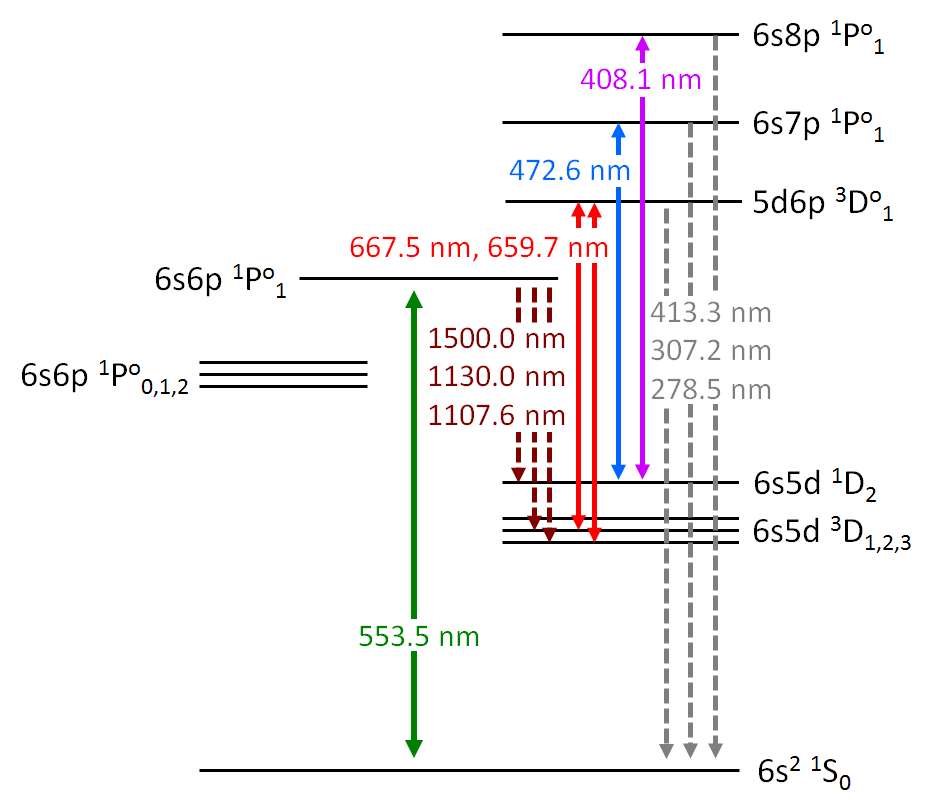
\includegraphics[width=.8\textwidth]{figures/elevs_Ba_extra.png}
	\caption{\emph{\color{gray}needs 3P to ground}Ba energy levels in vacuum.}
    \label{fig:elevsBa}
\end{figure}

The low-lying energy levels of Ba\textsuperscript{+} in vacuum are shown in Fig. \ref{fig:elevsBaPlus}.  Two strong transitions exist between the ground $6s$ $^{2}$S$_{1/2}$ state and the $6p$ $^{2}$P$_{1/2}$ and $6p$ $^{2}$P$_{3/2}$ excited states.  Branching ratios to the two metastable $^{2}$D states result in a decay into a $^{2}$D state after about 4 excitations.  Transition rates between these levels are listed in Table \ref{table:BaTransitions}.    

\begin{table}[!htbp]
\caption{Transition rates for the lowest-lying energy levels of Ba and Ba\textsuperscript{+} in vacuum.} %not sure what [Small Table], between \caption and {}, w/ no spaces, does
\label{table:BaTransitions}
\begin{tabular}{c|c|c c}
& Transition & Rate ($s^{-1}$) &  \\
\hline
Ba & $6s6p$ $^{1}$P$_{1}$\textsuperscript{o} $\rightarrow 6s^{2}$ $^{1}$S$_{0}$ & $1.19 \times 10^{8}$ & \cite{BaAllowedTransitions} \\
& $6s6p$ $^{1}$P$_{1}$\textsuperscript{o} $\rightarrow 6s5d$ $^{1}$D$_{2}$ & $2.50 \times 10^{5}$ & \cite{BaAllowedTransitions} \\
& $6s6p$ $^{1}$P$_{1}$\textsuperscript{o} $\rightarrow 6s5d$ $^{3}$D$_{2}$ & $1.1 \times 10^{5}$ & \cite{BaAllowedTransitions} \\
& $6s6p$ $^{1}$P$_{1}$\textsuperscript{o} $\rightarrow 6s5d$ $^{3}$D$_{1}$ & $3.1 \times 10^{3}$ & \cite{BaAllowedTransitions} \\
& $6s5d$ $^{1}$D$_{2} \rightarrow 6s^{2}$ $^{1}$S$_{0}$ & $4$ & \cite{Ba1D2and3D1} \\
& $6s5d$ $^{3}$D$_{2} \rightarrow 6s^{2}$ $^{1}$S$_{0}$ & $1.45 \time 10^{-2}$ & \cite{Ba3D2} \\
& $6s5d$ $^{3}$D$_{1} \rightarrow 6s^{2}$ $^{1}$S$_{0}$ & $1.7 \time 10^{-2}$ & \cite{Ba1D2and3D1} \\
& $6s6p$ $^{3}$P$_{1}$\textsuperscript{o} $\rightarrow 6s^{2}$ $^{1}$S$_{0}$ & {\color{red}???} & {\color{red}???}\\
\hline
Ba\textsuperscript{+} & $6p$ $^{2}P_{3/2}$\textsuperscript{o} $\rightarrow 6s $ $^{2}S_{1/2}$ & $1.11 \times 10^{8}$ & \cite{BaAllowedTransitions} \\
& $6p$ $^{2}P_{1/2}$\textsuperscript{o} $\rightarrow 6s$ $^{2}S_{1/2}$ & $9.53 \times 10^{7}$ & \cite{BaAllowedTransitions} \\
& $6p$ $^{2}P_{3/2}$\textsuperscript{o} $\rightarrow 5d$ $^{2}D_{5/2}$ & $4.12 \times 10^{7}$ & \cite{BaAllowedTransitions} \\
& $6p$ $^{2}P_{3/2}$\textsuperscript{o} $\rightarrow 5d$ $^{2}D_{3/2}$ & $6.00 \times 10^{6}$ & \cite{BaAllowedTransitions} \\
& $6p$ $^{2}P_{1/2}$\textsuperscript{o} $\rightarrow 5d$ $^{2}D_{3/2}$ & $3.10 \times 10^{7}$ & \cite{BaAllowedTransitions} \\
& $5d$ $^{2}D_{5/2} \rightarrow 6s$ $^{2}S_{1/2}$ & $3.8 \times 10^{-2}$ & \cite{BaPlusD52} \\
& $5d$ $^{2}D_{3/2} \rightarrow 6s$ $^{2}S_{1/2}$ & $1.3 \times 10^{-2}$ & \cite{BaPlusD32} \\
\end{tabular}
\end{table}

\begin{figure} %[H]
	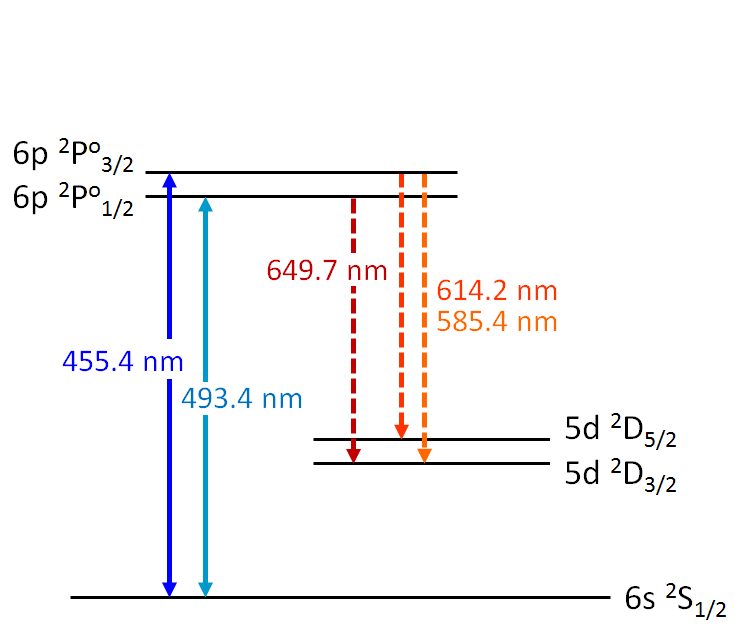
\includegraphics[width=.6\textwidth]{figures/elevs_Ba+_separate.png}
	\caption{Ba\textsuperscript{+} energy levels in vacuum.}
    \label{fig:elevsBaPlus}
\end{figure}

%These rates are shown in  along with each of the allowed transitions in Fig. \ref{fig:elevs}.

%The lowest-lying energy levels in vacuum for Ba and Ba\textsuperscript{+} are shown in Fig. \ref{fig:elevs}.  For Ba, the main transition is between the ground $6s^{2}$ $^{1}$S$_{0}$ to the excited $6s6p$ $^{1}$P$_{1}$\textsuperscript{o} state, however branching ratios from the P state result in a decay to one of three metastable D states in about 1 in 330 excitations.  For Ba\textsuperscript{+}, two strong transitions exist between the ground $6s$ $^{2}$S$_{1/2}$ and the $6p$ $^{2}$P$_{1/2}$ and $6p$ $^{2}$P$_{3/2}$ excited states.  Transitions to the two metastable D states are higher than for the atom, resulting in a decay into a D state after about 4 excitations.  These D states are metastable because they are parity-forbidden to decay back to the ground state, resulting in much lower decay rates.  These rates are shown in Table \ref{table:BaTransitions} along with each of the allowed transitions in Fig. \ref{fig:elevs}.

%\begin{figure}[H]
%	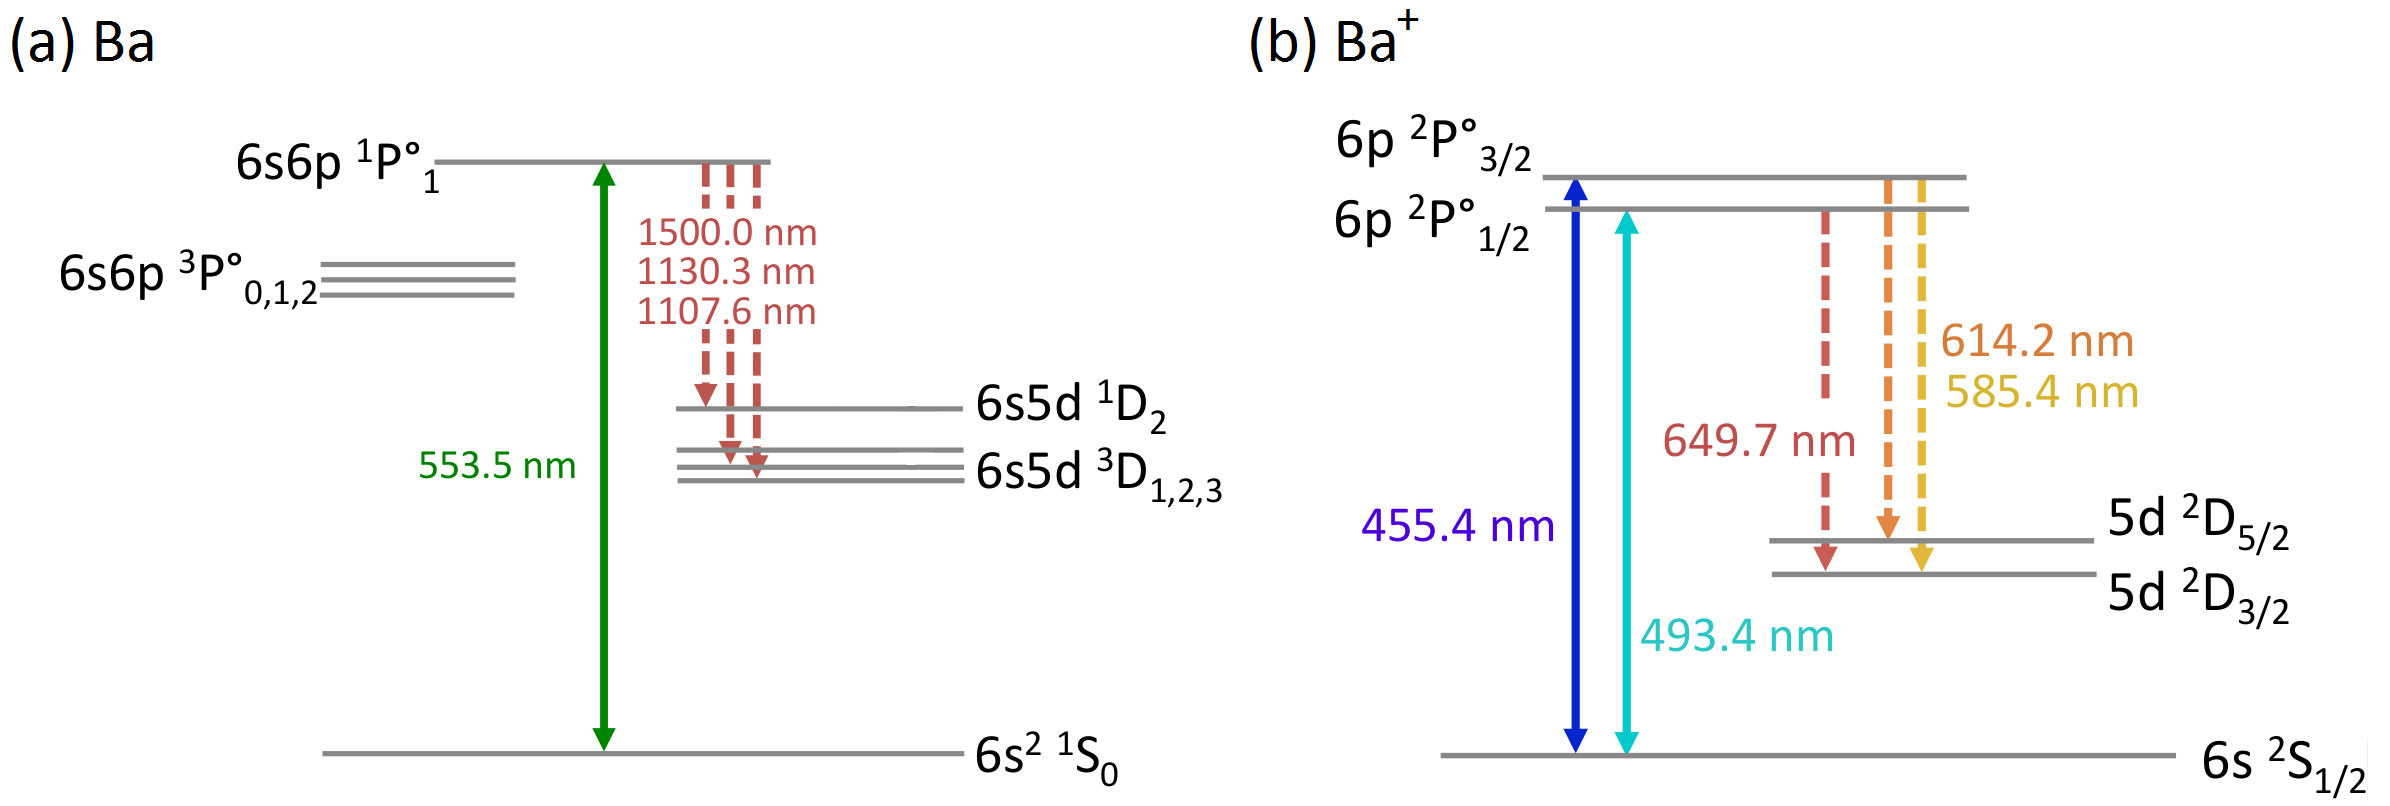
\includegraphics[width=.9\textwidth]{figures/elevs.png}
%	\caption{Energy level diagrams for (a) Ba and (b) Ba\textsuperscript{+}.}
%    \label{fig:elevs}
%\end{figure}

%These energy levels and their transition rates are well known, and are documented in the NIST Atomic Spectra Database.

Single atom/ion detection by spectroscopy requires many excitation/emission cycles in order to detect an observable number of photons from a single atom/ion.  For Ba/Ba\textsuperscript{+}, in addition to the main excitation laser, lasers may be needed to depopulate the metastable D states once the atom/ion becomes optically pumped into one of them.  This recovery is called re-pumping.  In Ba, re-pumping can be accomplished via three infrared lasers at wavelengths 1107.6~nm, 1130.0~nm, and 1500.0~nm for the direct transitions back to the $6s6p$ $^{1}$P$_{1}$\textsuperscript{o} state.  An alternative re-pumping scheme is via excitation to higher-level states which have paths back to the ground state or the $6s6p$ $^{1}$P$_{1}$\textsuperscript{o} state.  A few such higher-level re-pump transitions are shown in Fig. \ref{fig:elevsBa}, including two red transitions to the $5d6p$ $^{3}$D$_{1}$\textsuperscript{o}, and blue and violet transitions to the $6s7p$ $^{1}$P$_{1}$\textsuperscript{o} and $6s8p$ $^{1}$P$_{1}$\textsuperscript{o} states.  Trapping/detection of Ba atoms in a magneto-optical trap (MOT) was achieved in \cite{BaMOT}.  This was done with two separate re-pumping schemes:  by incorporating three infrared re-pump transitions, as well as with two infrared re-pump transitions along with a 659.7-nm laser re-pumping the $6s5d$ $^{3}$D$_{1}$ state via the $5d6p$ $^{3}$D$_{1}$\textsuperscript{o} state.  Observation of trapped single Ba\textsuperscript{+} ions in vacuum has been achieved using 493.4~nm along with one re-pump laser at 649.7~nm {\color{red}[???]}\cite{singleBaPlusEXO}.

%, replacing the 1130.6-nm transition directly to $6s6p$ $^{1}$P$_{1}$\textsuperscript{o}

\section{5-level System}
\label{sec:model}

The model for Ba transitions in vacuum with excitation to the $6s6p$ $^{1}$P$_{1}$\textsuperscript{o} state is a 5-level system, shown schematically in Fig. [].  States 1 and 2 represent the $6s^{2}$ $^{1}$S$_{0}$ and $6s6p$ $^{1}$P$_{1}$\textsuperscript{o} states, respectively, and states 3, 4 and 5 represent the $6s5d$ $^{1}$D$_{2}$, $6s5d$ $^{3}$D$_{2}$, and $6s5d$ $^{3}$D$_{1}$ states, respectively.  The rate equations for this system, neglecting stimulated emission, are:

% is stated in Eqn. \ref{eqn:rateEqn}:

\begin{equation}
\begin{aligned}
\frac{dN_1}{dt} &= - W_{12}N_{1} + A_{21}N_{2} + A_{31}N_{3} + A_{41}N_{4} + A_{51} N_{5} \\
\frac{dN_2}{dt} &= W_{12}N_{1} - N_{2}(A_{21} + A_{23} + A_{24} + A_{25}) \\
\frac{dN_3}{dt} &= A_{23}N_{2} - A_{31}N_{3} \\
\frac{dN_4}{dt} &= A_{24}N_{2} - A_{41}N_{4} \\
\frac{dN_5}{dt} &= A_{25}N_{2} - A_{51}N_{5} \\
\end{aligned}
\label{eqn:rateEqn}
\end{equation}

\noindent
where $N_{i}$ is the population in state $i$, $A_{ij}$ is the decay rate from state $i$ to state $j$, and $W_{12}$ is the excitation rate.

Under some experimental conditions, the assumption can be made that $W_{12}$ is small compared to the rates out of the $^{1}$P$_{1}$\textsuperscript{o} state.  In this case the population in the excited state $N_{2}$ is negligible.  For these conditions, there is an effective pumping rate for the D states:

\begin{equation}
W_{1i} = W_{12}\frac{A_{2i}}{A_{21} + A_{23} + A_{24} + A_{25}}
\label{eqn:smallW12pumpingRates}
\end{equation}

\noindent
where $i = 3,4,5$.  Eq. 8 is also true for $i = 1$, where $W_{11}$ represents the fluorescence rate.  The fraction in Eq. \ref{eqn:smallW12pumpingRates} is the respective branching ratio from the excited state.  With this definition, the rate equations for states 3, 4, and 5 can be re-written as:

%, including the pumping rate back to ground

\begin{equation}
\begin{aligned}
\frac{dN_3}{dt} &= W_{13}N_{1} - A_{31}N_{3} \\
\frac{dN_4}{dt} &= W_{14}N_{1} - A_{41}N_{4} \\
\frac{dN_5}{dt} &= W_{15}N_{1} - A_{51}N_{5} \\
\end{aligned}
\label{eqn:smallW12populationRates}
\end{equation}

\noindent
In the model, an additional variable is not needed for $N_{1}$.  Rather, $1 - N_{3} - N_{4} - N_{5}$ is used.  Beginning with all population in the ground state ($N_{3} = N_{4} = N_{5} = 0$), the model calculates the state populations $N_{i}$ at the end of each iterative time step, $t_{\text{step}}$, as:

\begin{equation}
\begin{aligned}
N_{i} = N_{i, previous} + \frac{dN_i}{dt}t_{\text{step}} \\
\end{aligned}
\label{eqn:smallW12populations}
\end{equation}

\noindent
where $i = 3,4,5$, and $dN_i/dt$ is determined at the beginning of each time step according to Eq. \ref{eqn:smallW12populationRates}.  Time steps of $t_{\text{step}} = 1~\mu$s were used.  In order to model data, which is taken in exposure time ($t_{\text{exp}}$) frames, the model iterates through $t_{\text{exp}}/t_{\text{step}}$ steps in each frame, accumulating fluorescence counts at each step ($C_{\text{step}}$) according to the fluorescence rate (Eq. \ref{eqn:smallW12pumpingRates} with $i = 1$) times $t_{\text{step}}$, amounting to:

\begin{equation}
\begin{aligned}
C_{\text{step}} = W_{12}\frac{A_{21}}{A_{21} + A_{23} + A_{24} + A_{25}}t_{\text{step}} \\
\end{aligned}
\label{eqn:smallW12counts}
\end{equation}

\noindent
To incorporate camera readout time, where laser exposure continues but fluorescence is not observed, populations and derivatives are iterated without adding to total counts.

\begin{figure} %[H]
        \centering
                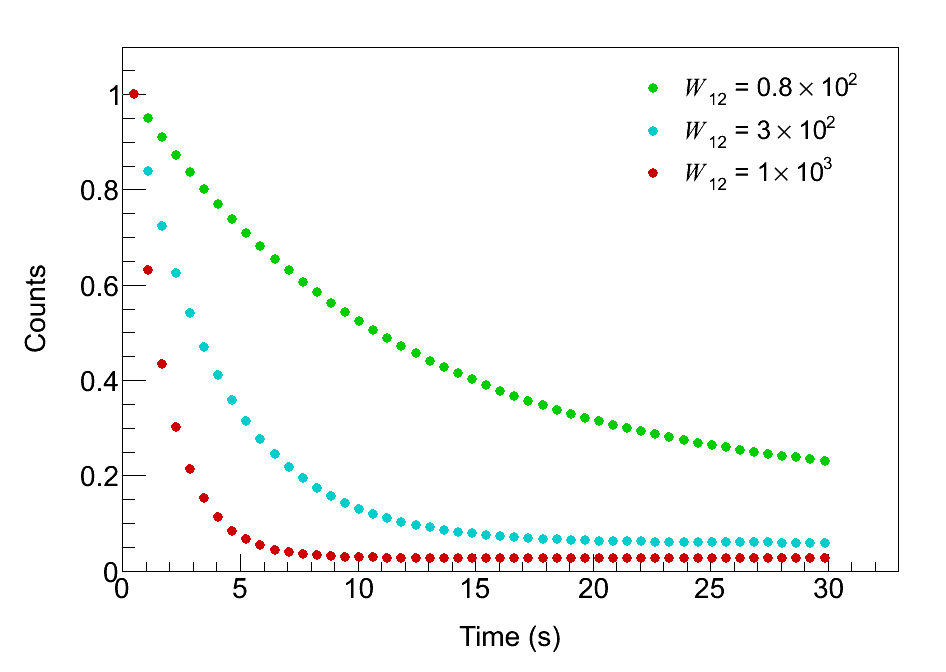
\includegraphics[width=.7\textwidth]{figures/thesis_modelExamples.png}
                \caption{Modeled counts in 0.5-s exposure frames for three values of $W_{12}$, using vacuum Ba transition rates, normalized to the first point.  Intermittent readout times of 0.1~s are used. }
\label{fig:modelExample}
\end{figure}

Examples of modeled counts vs. time are shown in Fig. \ref{fig:modelExample} for three values of $W_{12}$, using the transition rates of Ba in vacuum from Table \ref{table:BaTransitions}.  Decay of fluorescence occurs as atoms are optically pumped into the metastable D states.  This model is compared to bleaching data of Ba in SXe in Sec. \ref{sec:bleach577and591}.

%\begin{equation}
%\begin{aligned}
%\frac{dN_1}{dt} &= - w_{12}N_{1} + a_{21}N_{2} + a_{31}N_{3} %+ a_{41}N_{4} + a_{51} N_{5} + a_{61}N_{6} \\
%\frac{dN_2}{dt} &= w_{12}N_{1} - N_{2}(a_{21} + a_{23} + %a_{24} + a_{25} + a_{26}) \\
%\frac{dN_3}{dt} &= a_{23}N_{2} - a_{31}N_{3} \\
%\frac{dN_4}{dt} &= a_{24}N_{2} - a_{41}N_{4} \\
%\frac{dN_5}{dt} &= a_{25}N_{2} - a_{51}N_{5} \\
%\frac{dN_6}{dt} &= a_{26}N_{2} - a_{61}N_{6}
%\end{aligned}
%\label{eqn:rateEqn}
%\end{equation}

\section{Matrix Isolation Spectroscopy}
\label{sec:matrix}

%\emph{\color{gray}May be good matrix isolation theory references in Ba Spec... yeah, 1 and 2 i think ... shon's 55, 57, 58 are probably good too and maybe overlapping}

In the matrix isolation technique, a species of interest is trapped in a crystal, or ``matrix," of inert atoms/molecules such that it can be studied at leisure without guest-guest interactions.  To be effective, temperature must be low enough to prevent diffusion, and guest concentration must be low enough to prevent interaction.  The technique was originally proposed and demonstrated in \cite{matrixIso}, where short-lived species in chemical reactions were studied by isolating them in various solid matrices.  The proposed method of Ba tagging in SXe is a unique application of matrix isolation spectroscopy.  In order to understand the spectroscopic effects which may be encountered due to interaction between the guest Ba/Ba\textsuperscript{+} and the host Xe atoms, some effects encountered in systems of a metal atoms in rare-gas matrices are discussed.

%Low concentrations of the guest species, ideally at least 1:$10^{3}$ host:guest ratio, prevent guest-guest interactions.  

The leading interaction between a guest atom and host noble gas atoms is an induced dipole-dipole Van der Waals force.  For a metal atom of group I or II, this interaction is different when the atom is in the excited P state vs. the ground S state, resulting in general in a different potential energy relationship \cite{crepin}.  This can cause shifts and broadening of absorption and emission according to the Franck Condon Principle, illustrated in Fig. \ref{fig:FranckCondon} for the simple case of one-dimensional vibration between two bodies.  In a cold matrix, the system will be in the ground lattice vibrational state ($\nu =0$) before excitation.  Electronic excitation can occur to multiple vibrational modes whose wavefunctions overlap that of the ground state, thus broadening the absorption.  Absorption energy is determined by the difference in potential energy between the ground and excited states, which in general is not the same as the absorption energy in vacuum.  In the excited state, rapid decay occurs to the lowest vibrational mode, and then a similar broadening in the spontaneous emission energy occurs.  A redshift in the emission is observed relative to the excitation.  Additionally, splitting of orbital degeneracy in the P state can produce triplet structures in the absorption according to the Jahn-Teller effect \cite{jahnteller}.  These features depend on the specific configuration of atoms surrounding the guest, and thus different spectra can be observed from guest atoms occupying different matrix ``sites."  Diversity in matrix site populations from a deposit of many guest atoms can result in a multitude of emission peaks.  Annealing a matrix after deposition can reveal relative stability of various matrix sites \cite{crepin}.

%The ground S state of a group I or II atom is spherically symmetric, and being slightly larger in Van der Waals radius than Xe, it is likely to take the place of one or more Xe atoms in the fcc crystal (substitution), vs. existing in between Xe atoms in the crystal structure (interstitial).

%dynamic

%the strength of the Ba-Xe interaction, an induced dipole-dipole Van der Waals force, is quite different when the Ba is in the non-spherically-symmetric excited P state \cite{crepin}.  

% before electronic decay can occur

\begin{figure} %[H]
        \centering
                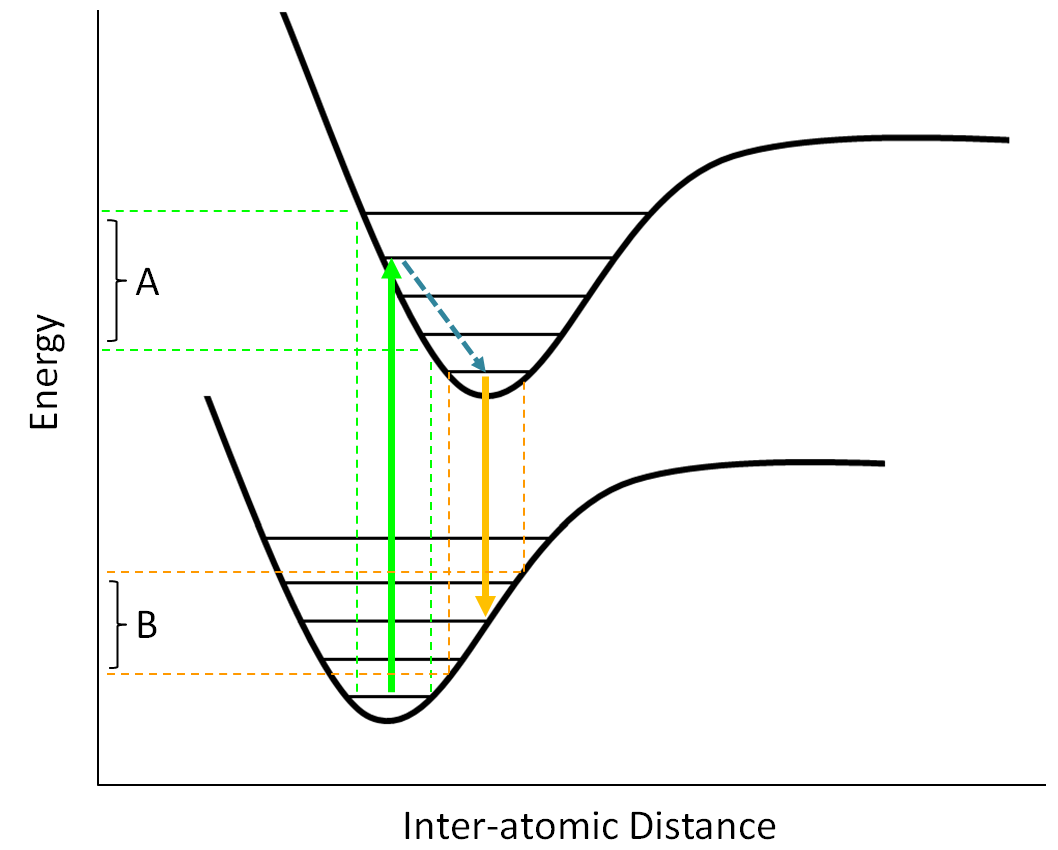
\includegraphics[width=.7\textwidth]{figures/FranckCondon.png}
                \caption{Illustration of the Franck-Condon Principle resulting in red-shifted emission as well as broadening in absorption (A) and emission (B) due to vibrational modes $\nu$ ($\nu$') in the ground (excited) state.}
\label{fig:FranckCondon}
\end{figure}

As an example, spectroscopy on Na atoms in solid rare-gas matrices is studied in \cite{matrixNa}.  Spectral features are exemplified in Fig. \ref{fig:matrixNa} for Na atoms in SAr, SKr, and SXe.  Excitation and emission are broadened to 10s of nm.  Two different matrix sites are observed in all three matrices, with the largest red-shift in emission observed in SXe.  The triplet structures in excitation spectra are attributed to the Jahn-Teller effect.

\begin{figure} %[H]
        \centering
                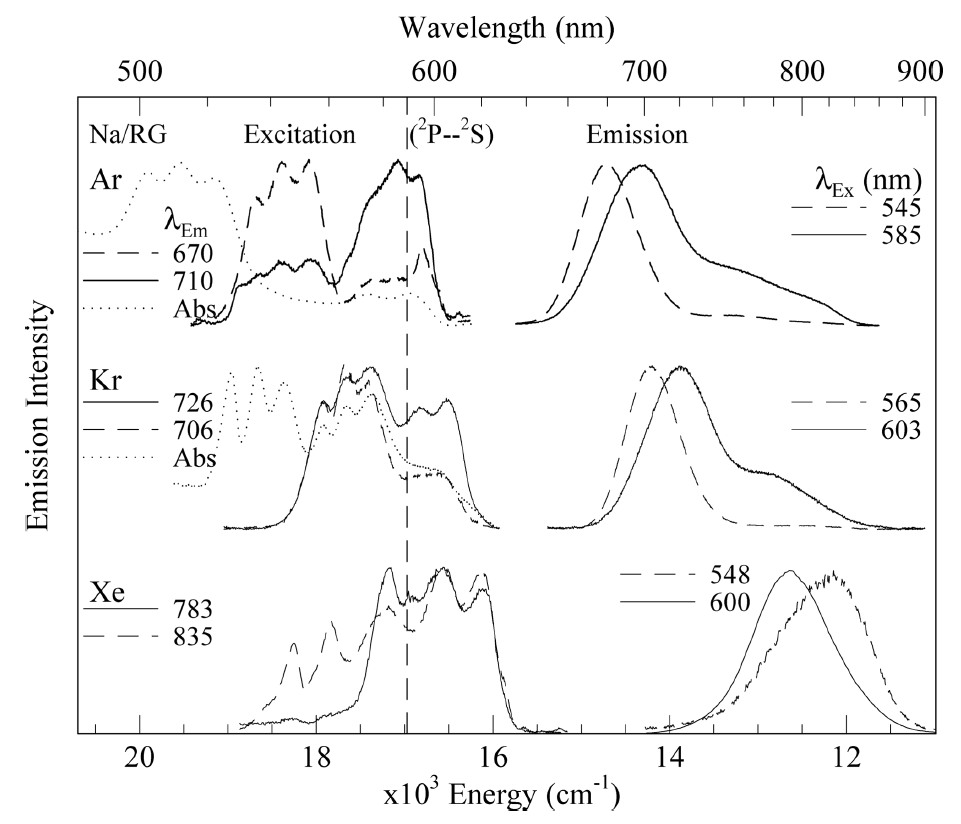
\includegraphics[width=.7\textwidth]{figures/Na_in_matrices.png}
                \caption{Excitation and emission spectra of Na atoms in SAr, SKr, and SXe.  \cite{matrixNa}}
\label{fig:matrixNa}
\end{figure}

%As as example \emph{\color{gray}is there a more modern example paper you can use?}, the spectroscopy of Ba in solid Ar (SAr) and solid Kr (SKr) matrices was studied in \cite{SAr}.  The example of Ba in SAr is shown in Fig. \ref{fig:BaSAr}.  The absorption is 10s of nm broad with a multi-peak structure, and the emission is broadened to nms and red-shifted.  These were attributed to the main $6s^{2}$ $^{1}$S$_{0} \rightarrow 6s6p$ $^{1}$P$_{1}$\textsuperscript{o} transition and its spontaneous emission. \emph{\color{gray}talk about other aspects.....brian says the triplet is caused by P state degeneracy being split, but I don't see how this makes sense, and also I have the impression that there are multiple explanations like Jahn Teller -- you should have a feel for this....}

%\begin{figure} %[H]
%        \centering
%                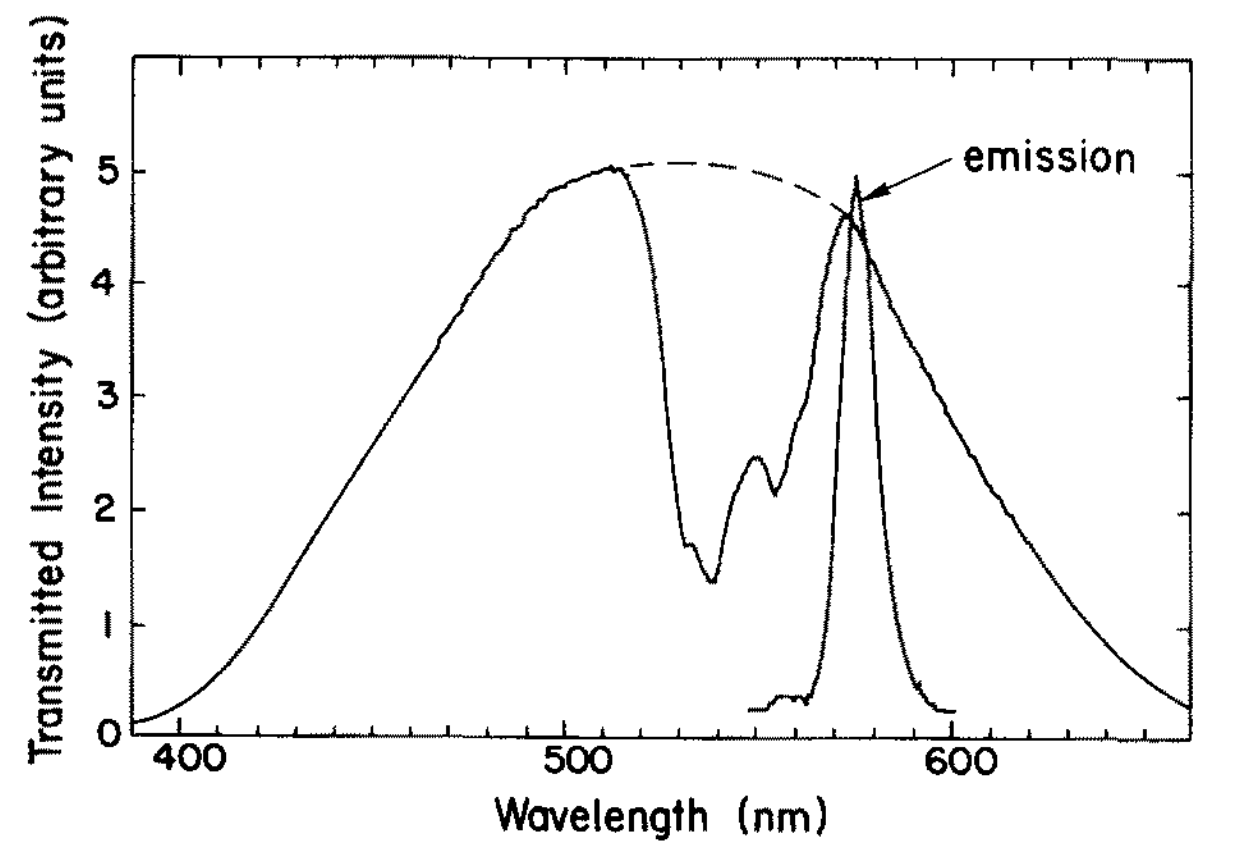
\includegraphics[width=.7\textwidth]{figures/Ba_in_SAr.png}
%                \caption{Absorption and emission spectra of neutral Ba in SAr at 10~K.  \cite{SAr}}
%\label{fig:BaSAr}
%\end{figure}

Energy level transition probabilities can also be affected in a matrix.  If potential energy curves cross each other, non-radiative transitions can become allowed for otherwise forbidden transitions \cite{crepin}.  Spin-forbidden transitions, both radiative and non-radiative, between triplet and singlet states can become more significant for heavy host atoms like Xe \cite{heavyAtom}.  Effects like these could aid in observation of the Ba/Ba\textsuperscript{+}, e.g. by improving decay rates out of metastable D states, or they could reduce detectability, e.g. if a non-radiative decay competes with the fluorescence channel.

%, e.g., spin-forbidden transitions can become more significant via the heavy atom effect [ref...i know you have crepin but maybe you can use crepin's ref, since you need to understand this anyway]

%The detectability of a single atom/ion can depend greatly on [these]...

\section{Fluorescence Efficiency}
\label{sec:fluorEff}

Fluorescence efficiency ($\epsilon_{f}$) is the ratio of fluorescence photons emitted to excitations into the fluorescing state.  This becomes less than one when there are paths out of the excited state other than the one which emits the photon being measured, e.g. the $\epsilon_{f}$ of Ba in vacuum is about 99.7\%, not quite 100\% due to about 1 in 330 decays from the P state into a metastable D state.  $\epsilon_{f}$ can be calculated by Eq. \ref{eqn:flueEff}:

\begin{equation}
\epsilon_{f} = \frac{f}{W_{12} \epsilon_{c}} = \frac{f h \nu}{\sigma I \epsilon_{c}}
\label{eqn:flueEff}
\end{equation}

\noindent
where $f$ is the number of fluorescence photons observed per atom per second, $W_{12}$ is the excitation rate, $\epsilon_{c}$ is the collection efficiency of the system, $\sigma$ is the cross section for the excitation interaction, $I$ is the laser intensity, and $h \nu$ is the excitation photon energy.  
%$\sigma$ can be measured by experiment, and the remaining parameters are easily calculated to produce a measurement of $\epsilon_{f}$.
% \emph{\color{gray}those statements are dumb, and do you want to ref brian for measuring the Ba $\sigma$?}.